\chapter{Introducción} 

\section{Caracterización acústica}

\subsection{Planteo físico y modelado por elementos finitos}

El experimento típico que se desea realizar consiste en estimular una respuesta de escape o sobresalto utilizando como fuente un parlante sumergido en la pecera. Una caracterización total de la acústica consistiría en:
\begin{itemize}
	\item La caracterización del parlante como emisor de sonido, principalmente la determinación de la direccionalidad de emisión.
	\item La caracterización de los campos acústicos dentro de la pecera, de presiones y de velocidades del medio (agua).
\end{itemize}
La caracterización del parlante requiere medir patrones de emisión en condiciones de campo libre donde los bordes de la pecera (o pileta) se encuentren a varias longitudes de onda del parlante; impracticable en una pecera de laboratorio. Para el estudio de los campos acústicos se requiere de hidrófonos (medidores de presión) y de un acelerómetro sumergible de alta presición. Inicialmente se planteó caracterizar ambos campos, pero el alto costo presupuestado para el acelerómetro (US\$5000) sólo permitió la caracterización del campo de presiones.

La onda sonora está completamente determinada por la ecuación de ondas de Helmholtz
\begin{equation}
	\nabla^2p(\vec{r})\,+\,\left(\frac{2\pi}{\lambda}\right)^2p(\vec{r})\,=\,0,
	\label{eq:helmholtz}
\end{equation}
la cual permite conocer el campo de presiones $p(\vec{r})$ para cualquier coordenada $\vec{r}$ dada la longitud de onda $\lambda$ (para aliviar la notación se han omitido las dependencias temporales en todas las fórmulas, y en lo siguiente también se omitirán las espaciales). Para completar la determinación del problema, se debe tener en cuenta que las partículas del medio se moverán siempre que se imponga un campo de presiones de gradiente no nulo. Las velocidades pueden obtenerse mediante aproximaciones de la ecuación de Navier-Stokes y la adición de una ecuación de estado:

\begin{align}
	\rho\,\frac{\partial\vec{u}}{\partial t}\,=\,-\vec{\nabla}p,
	\label{eq:stokes}\\
	p\,=\,c^2\,\rho '.
	\label{eq:fluidos}
\end{align}

Aquí, $\vec{u}$ es el campo de velocidades y $\rho$ la densidad estática del medio ($\approx$ 1g/m\textsuperscript{3} para el agua), $c$ es la velocidad de propagación del sonido en el medio ($\approx$ 1500m/s en agua) y $\rho'$ la densidad acústica.

La resolución de las ecuaciones \ref{eq:helmholtz}, \ref{eq:stokes} y \ref{eq:fluidos} no puede obtenerse en forma analítica y se debe recurrir a aproximaciones o métodos computacionales. En la bibliografía suelen encontrarse dos aproximaciones, la primera concierne a la ecuación de Helmholtz \ref{eq:helmholtz} y la segunda a las condiciones de borde.

En el rango de frecuencias de 20Hz hasta 20kHz las longitudes de onda en agua son de 0,75m hasta 75m, siendo los rangos de longitudes más grandes (menores frecuencias) los de mayor relevancia biológica. Esto implica que, en el caso más general, la longitud de onda es siempre mucho mayor que las medidas del acuario experimental (suelen ser del orden del metro) y la ecuación de Helmholtz \ref{eq:helmholtz} puede ser aproximada por la ecuación de Laplace:

\begin{equation}
	\vec{\nabla}p=0.
	\label{eq:laplace}
\end{equation} 

En cuanto a las condiciones de borde, en principio debería plantearse un cambio de medio en todas las superficies, agua-vidrio-aire para las paredes y agua-aire para la superficie libre. Sin embargo, los vidrios y plásticos utilizados en la construcción de peceras se doblan fácilmente con las presiones acústicas, y aún cerca de las paredes existe movimiento de partículas. Esto quiere decir que, a primer orden, el acuario se comporta como un bloque de agua aislado con condiciones de bordes suave (pressure release). Si la fuente de sonido está dentro del agua, la presión se anula en todas las superficies pero los campos de velocidades no. Estas condiciones, opuestas a las utilizadas generalmente en aire (bordes duros, velocidad nula en interfaces) son las que le dan complejidad al problema.

Utilizando las aproximaciones discutidas, se pueden derivar de la ecuación de Laplace \ref{eq:laplace} las frecuencias de los modos resonantes \emph{sólo del agua}. Esto es, aquellos modos que no se deban a la interacción con el material del acuario. Dichas frecuencias están dadas por la ecuación [1]
\begin{equation}
	f_{lmn}\,=\,\frac{c}{2}\sqrt{\frac{l}{L^2_x}\,+\,\frac{l}{L^2_y}\,+\,\frac{l}{L^2_z}},
	\label{eq:resonancias}
\end{equation}
donde $l$, $m$ y $n$ se refieren al número de modo y $L_x$, $L_y$ y $L_z$ son las dimensiones del acuario.

La mayoría de los estudios bibliográficos utilizan las aproximaciones discutidas y no tienen en cuenta la interacción del agua con el aire ni el vidrio [2, 3]. Con el objetivo de realizar un estudio más completo se recurrió al análisis por elementos finitos mediante el software COMSOL Multiphysics\textregistered 5.2.

Se programó un modelo del acuario en COMSOL y se exploraron distintas condiciones de borde, rodeando a la pecera con una capa perfectamente acoplada (perfectly matched layer) que simula al aire circundante.  Modelar las interfases como borde suave da lugar a resultados que concuerdan con las aproximaciones discutidas y los resultados que se obtienen de las ecuaciones \ref{eq:laplace} y \ref{eq:resonancias}. Se decidió, guiado en parte por resultados obtenidos, modelar sólo las interfases agua-vidrio como bordes suave y dejar la superficie libre del acuario como una discontinuidad en el medio de propagación (agua-aire). Con esas condiciones de borde, el programa calcula en forma numérica los campos de presiones en toda la pecera para distintas frecuencias en el rango de 400Hz hasta 10kHz. Como fuente de sonido se utiliza un emisor de ondas planas de geometría cilíndrica; ubicado en el mismo lugar donde se coloca el parlante en los experimentos.

\subsection{Caracterización mediante respuestas impulso}
\label{sec:introsweeps}

Para comparar el modelado numérico con la realidad del experimento, debe medirse la respuesta del acuario a todas las frecuencias utilizadas y en todos los puntos calculados. Este método de caracterización implica una cantidad de tiempo significativa para las condiciones experimentales trabajadas, pero se pueden obtener relaciones señal-ruido enormes debido a la concentración de energía en una sóla frecuencia. Sin embargo, existen otras complicaciones: en la práctica, todos los amplificadores y el parlante utilizado producen distorsión armónica. Esto quiere decir que al querer emitir un tono puro de frecuencia definida, inevitablemente se emitirán también tonos de frecuencias más altas. Para analizar estas mediciones se debe filtrar y rectificar la frecuencia fundamental o procesar la señal mediante transformadas de Fourier y obtener la fundamental a partir del espectro. Ambos métodos son complicados en cuanto al setup a utilizar: el primero requiere de filtros pasa banda de alta precisión y selectividad, mientras que el segundo sólo es posible mediante la generación digital de la señal y la sincronización del conversor DA del emisor y el AD del receptor. 

Es por eso que, en general, siempre es preferible recurrir a la determinación de la \emph{respuesta impulso} (RI). La RI de un sistema acústico es la respuesta del sistema a una pequeña perturbación de duración breve (un impulso, teóricamente una delta de Dirac). En acústica y procesamiento de señales la RI es una función temporal, $h(t)$, que al ser convolucionada con una perturbación cualquiera, $x(t)$, da como resultado la respuesta $y(t)$ del sistema al estímulo:

\begin{equation}
	y(t)\,=\,h(t)\,\otimes\,x(t).
\end{equation}

Para sistemas lineales y temporalmente invariantes, la transformada de la respuesta impulso es la función transferencia del sistema en el espacio de frecuencias. Por esta razón, si se logra medir y calcular la RI  del sistema, el mismo quedará completamente determinado.

El método generalmente elegido consiste en excitar al sistema con un barrido en frecuencias (señal de prueba) y obtener la RI mediante una deconvolución aperiódica con un filtro acorde (filtro inverso). En el espacio temporal, la señal de prueba se define como
\begin{equation}
	x(t)\,=\,\sin
	\left\lbrace
	\frac{w_1\,T}{\ln \left(\frac{\omega_2}{\omega_1}\right)}\,
	\left[\exp 
			\left(\frac{t}{T}\ln \left(\frac{\omega_2}{\omega_1}\right)
	\right)\,-\,1\right]
	\right\rbrace,
\end{equation}
y es un barrido que empieza a la frecuencia angular $\omega_1$, y termina a la frecuencia $\omega_2$ después de $T$ segundos. En la práctica, la señal de prueba se genera programando el espectro en el espacio de las frecuencias con un retardo de grupo\footnote{El retardo de grupo es el retardo temporal de la envolvente de la señal, \emph{no es un retardo de fase.}} que incremente en forma logarítmica. Las formulaciones pertinentes a la generación del barrido pueden encontrarse en [4] y una introducción larga y amena al método en [5]. Un espectrograma de una señal de prueba puede observarse en la figura \ref{fig:testsweep}.

\begin{figure}[H]
	\centering
		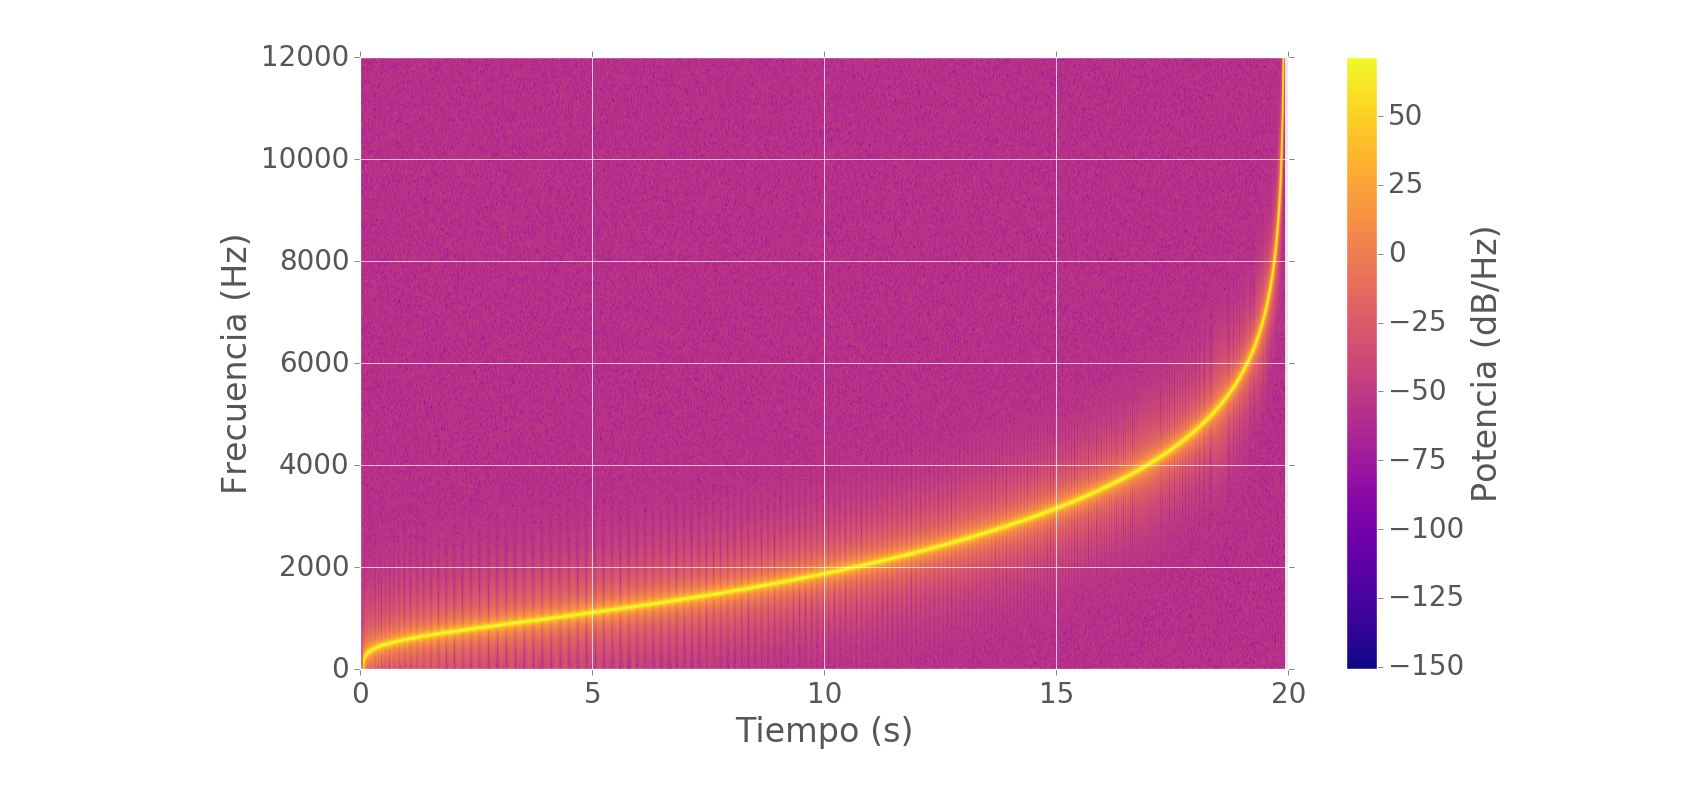
\includegraphics[scale=.43]{testsweep.png}
		\caption{Señal de prueba generada en el espacio de frecuencias. La linea amarilla representa una función senoidal cuya frecuencia varía en forma exponencial en función del tiempo. La frecuencia sube rápidamente desde 0Hz hasta 400Hz, donde inicia el barrido exponencial hasta 10kHz (luego sube rápidamente hasta la mitad de la frecuencia de muestreo con la que se generó la señal de prueba).}
	\label{fig:testsweep}
\end{figure}

Usualmente, como se muestra en la figura \ref{fig:testrec}, la grabación de la señal de prueba traerá consigo distorsiones armónicas (sobretonos de la señal original). La gran ventaja del método frente a otros existentes es que, si la distorisón armónica no es demasiado grande, se puede separar completamente la RI (\emph{respuesta lineal} del medio) de la distorsión armónica (producida por no linealidades en amplificadores y parlantes). 

\begin{figure}[H]
	\centering
		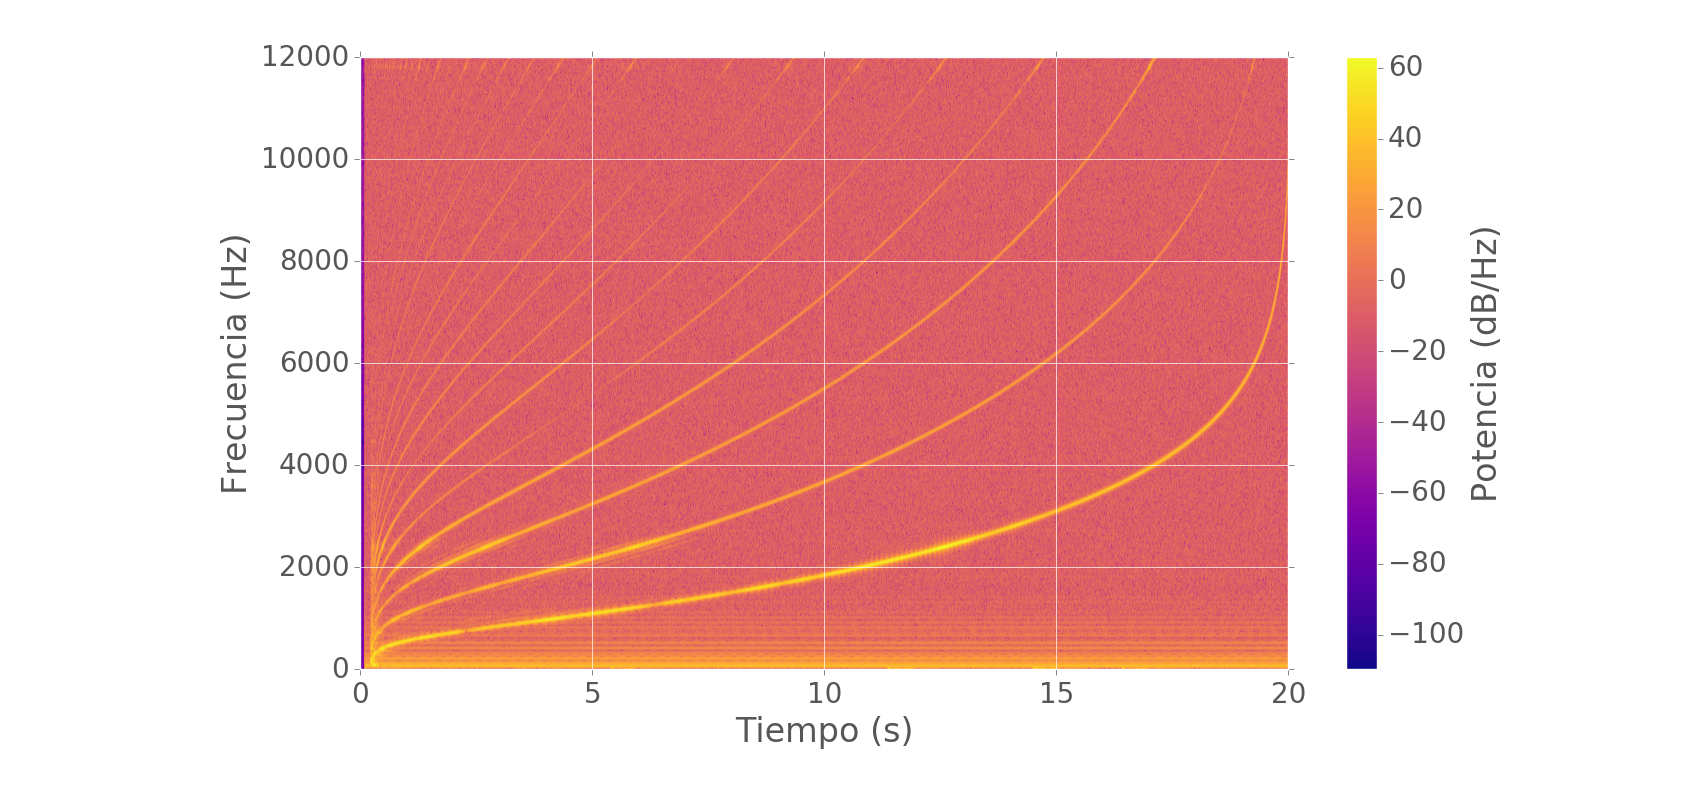
\includegraphics[scale=.43]{testrec.png}
		\caption{Grabación de la señal de prueba en una pecera. Se observan las frecuencias de la señal original y las distorsiones armónicas cuyas frecuencias son múltiplos enteros de las frecuencias originales.}
	\label{fig:testrec}
\end{figure}

El proceso de deconvolución y separación se explica con el siguiente ejemplo: para comprimir una señal de prueba que pase por 100Hz a los 100ms y 200Hz a 200ms el filtro inverso debe tener un retardo de grupo de -100ms a 100Hz y -200ms a 200Hz. Si el sistema analizado presenta armónicos de segundo orden al pasar por 100Hz, estos serán tratados con el retardo de grupo de -200ms, apareciando en la señal convolucionado a tiempo -100ms. Distorsiones de ordenes mayores aparecerán en momentos aún más negativos. La figura \ref{fig:x1y10} muestra la RI obtenida a partir de la deconvolución de la señal grabada en la figura \ref{fig:testrec}. La barra vertical de alta intensidad al comienzo es la RI: todas las frecuencias encendidas a la vez. Los rulos que se observan al costado son efecto de la distorsión armónica demasiado grande y la circularidad de la FFT en el algoritmo de procesado.

\begin{figure}[H]
	\centering
		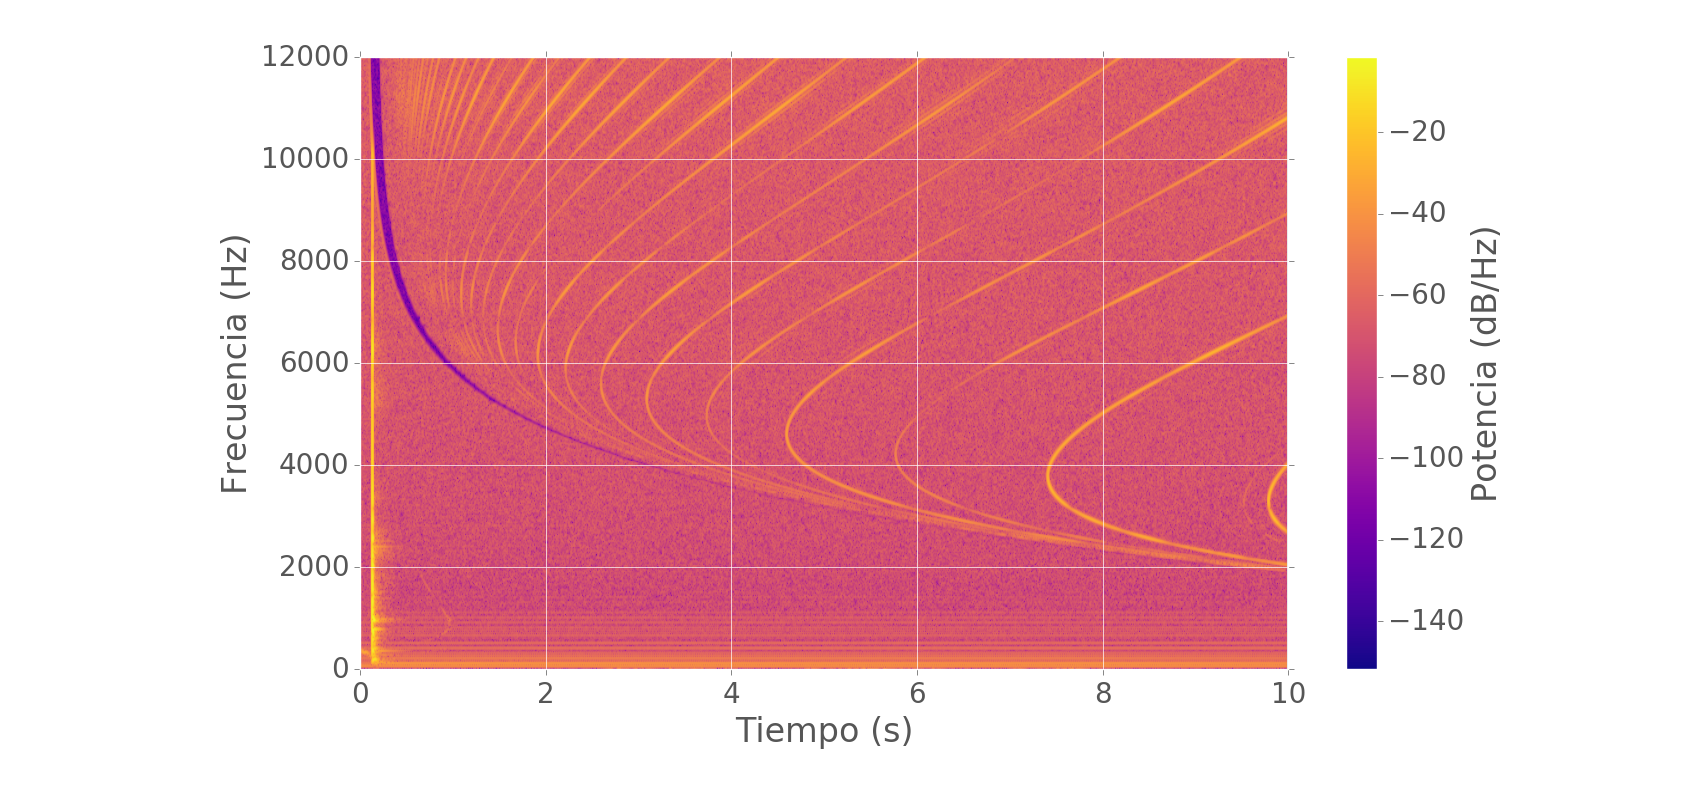
\includegraphics[scale=.43]{x1y10.png}
		\caption{RI de la señal de prueba con distorsión armónica obtenida mediante deconvolución con el filtro inverso.}
	\label{fig:x1y10}
\end{figure}

Los cálculos realizados por COMSOL dan la respuesta (compleja) de la pecera para distintas frecuencias, i.e. una amplitud compleja para cada punto del acuario como respuesta a un forzante armónico de frecuencia única. Realizando los calculos en un rango amplio de frecuencias, se puede obtener (mediante la transformada inversa de Fourier) la respuesta impulso en cada punto de la pecera.

La caracterización y modelado se hizo sobre la pecera con el parlante y luego se realizaron caracterizaciones de la pecera conteniendo una goma de neoprene que sirve de aislante.